%
%  untitled
%
%  Created by Parham Aram on 2010-07-14.
%  Copyright (c) 2010 . All rights reserved.
%
\documentclass[]{article}

% Setup for fullpage use
\usepackage{fullpage}

\usepackage[pdftex]{graphicx}


% More symbols
\usepackage{amsmath}
\usepackage{amssymb}

\usepackage[usenames,dvipsnames]{color}
\newcommand{\dean}[1]{\textcolor{red}{#1}}
\newcommand{\parham}[1]{\textcolor{blue}{#1}}

\begin{document}


\renewcommand{\theequation}{S1.\arabic{equation}}


\subsection*{Estimation of Connectivity Kernel Support}
The support of the connectivity kernel can be inferred using spatial correlation analysis. The method presented in this paper is based on a similar published method, where the kernel support was estimated using correlation analysis for a linear system described by an IDE~\cite{Scerri2009}. To demonstrate the method for the neural field model we assume the sensors are infinitesimally close (continuous observation). The spatial cross-correlation function between consecutive observations is defined as 
\begin{align}
	R_{y_{t},y_{t+1}}(\boldsymbol{\tau}) &= \mathbf{E}\left[ y_{t}\left(\mathbf{r}\right) y_{t+1}\left(\mathbf{r}+\boldsymbol{\tau}\right) \right] \\
	&= \mathbf{E}\left[\left(\left(m\ast v_t\right)\left(\mathbf{r}\right) + \boldsymbol{\varepsilon}_t\left(\mathbf{r}\right) \right) \times \left(\left( m \ast v_{t+1}\right)\left(\mathbf{r}+\boldsymbol{\tau}\right)+ \boldsymbol{\varepsilon}_{t+1}\left(\mathbf{r}+\boldsymbol{\tau}\right)\right) \right], \label{eq:ObsXCorr}
\end{align}

where $\mathbf{E}[\cdot]$ is the expected value. Since the observation noise is zero mean, temporally white and independent of the field, equation~\ref{eq:ObsXCorr} reduces to
\begin{equation}
	R_{y_{t},y_{t+1}}(\boldsymbol{\tau}) = \mathbf{E}\left[ \left(m \ast v_t\right)\left(\mathbf{r}\right) \times \left(m \ast v_{t+1}\right)\left(\mathbf{r}+\boldsymbol{\tau}\right)\right].
\end{equation}
Substituting in equation~\ref{DiscreteTimeModel}  for $v_{t+1}\left(\mathbf{r}\right)$, the cross-correlation function is
\begin{align}
	R_{y_{t},y_{t+1}}(\boldsymbol{\tau}) &= \mathbf{E}\left[ \left(m \ast v_t \right)\left(\mathbf{r}\right) \times m\left(\mathbf{r}+\boldsymbol{\tau}\right) \ast \left( \xi v_t\left(\mathbf{r}+\boldsymbol{\tau}\right) + T_s w\left(\mathbf{r}+\boldsymbol{\tau}\right) \ast f\left(v_t\left(\mathbf{r}+\boldsymbol{\tau}\right)\right) + e_t\left(\mathbf{r}+\boldsymbol{\tau}\right)\right) \right] \nonumber \\	
	 &= \xi \mathbf{E}\left[ \left(m \ast v_t \right)\left(\mathbf{r}\right) \times \left(m \ast v_t\right)\left(\mathbf{r}+\boldsymbol{\tau}\right)\right] \nonumber \\
	&+ T_s\mathbf{E}\left[\left(m \ast v_t \right)\left(\mathbf{r}\right) \times \left(m \ast w \right)\left(\mathbf{r}+\boldsymbol{\tau}\right) \ast f\left(v_t\left(\mathbf{r}+\boldsymbol{\tau}\right)\right) \right] \nonumber \\
	&+ \mathbf{E}\left[ \left(m \ast v_t \right)\left(\mathbf{r}\right)  \times \left(m \ast e_t\right)\left(\mathbf{r}+\boldsymbol{\tau}\right)\right] \nonumber \\
	&= R_1(\boldsymbol{\tau}) + R_2(\boldsymbol{\tau}) + R_3(\boldsymbol{\tau}).\label{eq:spatialxcorr} 
\end{align}
For simplicity we use $z_{t}\left(\mathbf{r}\right)$ to denote noise free observations, i.e.,
\begin{align}
z_{t}\left(\mathbf r\right)&=\left(m\ast v_{t}\right)\left(\mathbf{r}\right). 
\end{align}
The first term, $R_1(\boldsymbol{\tau})$, can be simplified to (assuming $\tau$ is a discrete variable)
\begin{align}
	R_1(\boldsymbol{\tau}) &= \xi \mathbf{E}\left[z_{t}\left(\mathbf r\right)  z_{t}\left(\mathbf{r}+\boldsymbol{\tau}\right) \right] \\
	&= \xi\left( R_{y_{t},y_{t}}(\boldsymbol{\tau}) - \sigma_{\varepsilon}^2\delta_K\left(\boldsymbol{\tau}\right) \right). \label{eq:R1}
\end{align}
% The second term
% \begin{equation}
% 	R_2(\boldsymbol{\tau}) = T_s\mathbf{E}\left[ m\left(\mathbf{r}\right) \ast v_t\left(\mathbf{r}\right) \times m\left(\mathbf{r}+\boldsymbol{\tau}\right) \ast w\left(\mathbf{r}+\boldsymbol{\tau}\right) \ast f\left(v_t\left(\mathbf{r}+\boldsymbol{\tau}\right)\right) \right]
% \end{equation}
Now we assume that the sigmoid activation function, $f(\cdot)$, can be approximated by the piecewise function
\begin{equation}
	\hat{f}(v_t(\mathbf{r}')) = \left\{ \begin{array}{ll}
		0, & v_t(\mathbf{r}') \le v_1 \\
		\varsigma v_t(\mathbf{r}'), &  v_1 < v_t(\mathbf{r}') < v_2 \\
		1, & v_t(\mathbf{r}') \ge v_2 \\ 
		\end{array}\right.
\end{equation}
Furthermore, we assume the field is in the linear region of the piecewise function for the majority of the time giving
\begin{equation}
	R_2(\boldsymbol{\tau}) \approx T_s \varsigma \mathbf{E}\left[ z_{t}\left(\mathbf{r}\right)\times \left(z_{t} \ast w\right)\left(\mathbf{r}+\boldsymbol{\tau}\right)\right].
\end{equation}
$R_2(\boldsymbol{\tau})$ can be written as
\begin{align}
	R_2(\boldsymbol{\tau}) &\approx T_s \varsigma \mathbf{E}\left[ z_{t}\left(\mathbf{r}\right)  \int_{\Omega}z_{t}\left(\mathbf{r'}\right) w\left(\mathbf{r}+\boldsymbol{\tau}-\mathbf{r'}\right) d\mathbf{r'} \right] \\
	&= T_s \varsigma \mathbf{E}\left[  \int_{\Omega}z_{t}\left(\mathbf{r}\right)z_{t}\left(\mathbf{r'}\right) w\left(\mathbf{r}+\boldsymbol{\tau}-\mathbf{r'}\right) d\mathbf{r'} \right] \\
	&= T_s \varsigma \mathbf{E}\left[  \int_{\Omega}z_{t}\left(\mathbf{r}\right)z_{t}\left(\mathbf{r}+\mathbf{r'}\right) w\left(\boldsymbol{\tau}-\mathbf{r'}\right) d\mathbf{r'} \right] \\
	&= T_s \varsigma   \int_{\Omega}\mathbf{E}\left[z_{t}\left(\mathbf{r}\right)z_{t}\left(\mathbf{r}+\mathbf{r'}\right) \right] w\left(\boldsymbol{\tau}-\mathbf{r}'\right) d\mathbf{r'}  \\
	&= \frac{T_s \varsigma}{\xi} \int_{\Omega} R_1(\mathbf{r'}) w\left(\boldsymbol{\tau}-\mathbf{r}'\right) d\mathbf{r'}  \\
	&= \frac{T_s \varsigma}{\xi} \left(R_1 \ast w\right)\left(\boldsymbol{\tau}\right)\\
\end{align}
The last term on the right hand side of equation~\ref{eq:spatialxcorr} is
\begin{equation}
	R_3(\boldsymbol{\tau}) = 0,
\end{equation}
since the disturbance added to the field at time $t$ and assumed to be uncorrelated to the field at time $t$. Therefore 
\begin{equation}
	R_{y_{t},y_{t+1}}(\boldsymbol{\tau}) - R_1(\boldsymbol{\tau}) \approx \frac{T_s \varsigma}{\xi} \left(R_1 \ast w\right)\left(\boldsymbol{\tau}\right).
\end{equation}
Now we rewrite this equation as a matrix convolution giving
\begin{equation}
	\mathbf{y} = \mathbf{A}\mathbf{x}
\end{equation}

Now, by taking the Fourier transform we get
\begin{equation}
	\mathcal{F}\left\{ R_{y_{t},y_{t+1}}(\boldsymbol{\tau}) - R_1(\boldsymbol{\tau}) \right\} \approx \frac{T_s \varsigma}{\xi} \mathcal{F} \left\{ R_1(\boldsymbol{\tau}) \right\} \mathcal{F}\left\{ w\left(\boldsymbol{\tau}\right)\right\}.
\end{equation}
% This simplifies to (\dean{this step is where need to find a better method for deconv})
% \begin{align}
% 	\Delta^2&\sum_{\tau_{min}}^{\tau_{max}}\sum_{\tau_{min}}^{\tau_{max}}\left(R_{y_{t},y_{t+1}}(\boldsymbol{\tau}) - R_1(\boldsymbol{\tau})\right) \exp\left(-j2\pi f \tau_x T_s\right)\exp\left(-j2\pi f \tau_y T_s\right) \\
% 	& \approx \Delta^2\sum_{\tau_{min}}^{\tau_{max}}\sum_{\tau_{min}}^{\tau_{max}} R_1(\boldsymbol{\tau}) \exp\left(-j2\pi f \tau_x T_s\right)\exp\left(-j2\pi f \tau_y T_s\right) \\
% 	&\times \Delta^2\sum_{\tau_{min}}^{\tau_{max}}\sum_{\tau_{min}}^{\tau_{max}} w(\boldsymbol{\tau}) \exp\left(-j2\pi f \tau_x T_s\right)\exp\left(-j2\pi f \tau_y T_s\right)
% \end{align}

\begin{equation}
	\frac{\xi}{T_s \varsigma} \left(\frac{\mathcal{F}\left\{R_{y_{t},y_{t+1}}(\boldsymbol{\tau})\right\}}{\mathcal{F}\left\{R_1(\boldsymbol{\tau})\right\}} - 1\right) \approx  W\left(\boldsymbol{\nu}\right).
\end{equation}
Now substituting back in equation~\ref{eq:R1}, we can write

\begin{align}
	W\left(\boldsymbol{\nu}\right) &\approx \frac{\xi}{T_s \varsigma} \left(\frac{\mathcal{F}\left\{R_{y_{t},y_{t+1}}(\boldsymbol{\tau})\right\}}{\xi\mathcal{F}\left\{\left( R_{y_{t},y_{t}}(\boldsymbol{\tau}) - \sigma_{\varepsilon}^2\delta_K\left(\boldsymbol{\tau}\right) \right)\right\}} - 1\right)  \\
	&= \frac{1}{T_s \varsigma} \left(\frac{\mathcal{F}\left\{R_{y_{t},y_{t+1}}(\boldsymbol{\tau})\right\}}{\mathcal{F}\left\{ R_{y_{t},y_{t}}(\boldsymbol{\tau})\right\} - \sigma_{\varepsilon}^2 } - \xi\right) \\
	&= \frac{1}{T_s \varsigma} \left(\frac{S_{y_{t},y_{t+1}}\left(\boldsymbol{\nu}\right)}{S_{y_{t},y_{t}}\left(\boldsymbol{\nu}\right) - \sigma_{\varepsilon}^2 } - \xi\right)
\end{align}

This equation states that the support of the kernel can be estimated given knowledge of $\sigma_\varepsilon^2$. The other parameters simply give an offset and scale the kernel. Furthermore, if we guess $\sigma_\varepsilon^2$ incorrectly, then the effect will only appear at $\boldsymbol{\tau}=0$. So if we assume local excitation, then we do not need to know $\sigma_\varepsilon^2$.\\


% We can also write an alternative less simplified form 
% \begin{equation}
% 	R_2(\boldsymbol{\tau}) \approx T_s \varsigma (R_{y_{t},y_{t}}(\boldsymbol{\tau}) - \sigma_{\varepsilon}^2\delta_K\left(\boldsymbol{\tau}\right)) \ast w(\boldsymbol{\tau})  
% \end{equation}
% 
% 
% \begin{align}
% 	R_2(\boldsymbol{\tau}) &\approx R_{y_{t},y_{t+1}}(\boldsymbol{\tau}) - R_1(\boldsymbol{\tau}) \\
% 	T_s \varsigma (R_{y_{t},y_{t}}(\boldsymbol{\tau}) - \sigma_{\varepsilon}^2\delta_K\left(\boldsymbol{\tau}\right)) \ast w\left(\boldsymbol{\tau}\right) &\approx R_{y_{t},y_{t+1}}(\boldsymbol{\tau}) - \xi\left( R_{y_{t},y_{t}}(\boldsymbol{\tau}) - \sigma_{\varepsilon}^2\delta_K\left(\boldsymbol{\tau}\right))  \right)
% \end{align}
% Take FFT of both sides
% \begin{align}
% 	T_s \varsigma (S_{y_{t},y_{t}}\left(\boldsymbol{\nu}\right) - \sigma_{\varepsilon}^2) W\left(\boldsymbol{\nu}\right) &\approx S_{y_{t},y_{t+1}}\left(\boldsymbol{\nu}\right) - \xi (S_{y_{t},y_{t}}\left(\boldsymbol{\nu}\right) - \sigma_{\varepsilon}^2) \\
% 	W\left(\boldsymbol{\nu}\right) &\approx \frac{S_{y_{t},y_{t+1}}\left(\boldsymbol{\nu}\right) - \xi (S_{y_{t},y_{t}}\left(\boldsymbol{\nu}\right) - \sigma_{\varepsilon}^2)}{T_s \varsigma (S_{y_{t},y_{t}}\left(\boldsymbol{\nu}\right) - \sigma_{\varepsilon}^2)}
% \end{align}

\begin{figure}[!ht]
\begin{center}
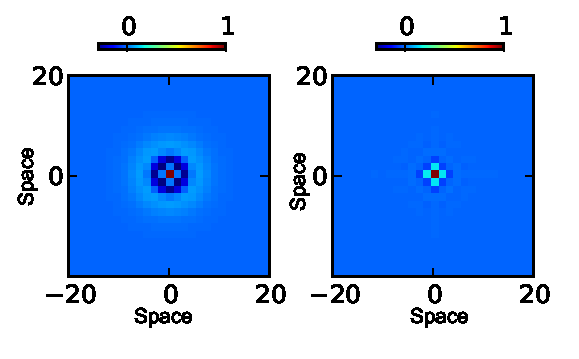
\includegraphics{./Figures/KernelWidthEstimation.pdf}
\end{center}
\caption{{\bf Estimation of Connectivity Kernel Support}. The kernel values are normalised. True  and estimated kernels are shown with solid and dotted lines respectively.}
\label{fig:KernelWidth}
\end{figure}

\begin{figure}[!ht]
\begin{center}
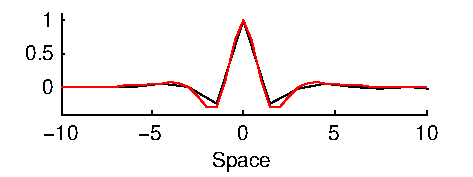
\includegraphics{./Figures/KernelWidthEstimation2.pdf}
\end{center}
\caption{{\bf Estimation of Connectivity Kernel Support}. The kernel values are normalised. True  and estimated kernels are shown with black and red lines respectively.}
\label{fig:KernelWidth2}
\end{figure}

% \newpage
% 
% \subsection*{CRAZY}
% \begin{align}
% 	R_{v_{t+1}v_t}(\boldsymbol{\tau}) &= \int_{\Omega} v_{t+1}(\mathbf{r}) v_t(\mathbf{r}+\boldsymbol{\tau}) d\mathbf{r} \\
% 	&= \int_{\Omega} \left(\xi v_t(\mathbf{r}) + g_t(\mathbf{r}) + e_t(\mathbf{r})\right) v_t(\mathbf{r}+\boldsymbol{\tau}) d\mathbf{r} \\
% 	&= \xi \int_{\Omega} v_t(\mathbf{r}) v_t(\mathbf{r}+\boldsymbol{\tau})d\mathbf{r} + \int_{\Omega}g_t(\mathbf{r})v_t(\mathbf{r}+\boldsymbol{\tau}) d\mathbf{r} + \int_{\Omega} e_t(\mathbf{r})v_t(\mathbf{r}+\boldsymbol{\tau})d\mathbf{r}
% \end{align}
% These four terms in the above equation are easy to compute and it all balances. From this we can write
% \begin{equation}
% 	R_{v_{t+1}v_t}(\boldsymbol{\tau}) - \xi R_{v_tv_t}(\boldsymbol{\tau}) = \int_{\Omega}g_t(\mathbf{r})v_t(\mathbf{r}+\boldsymbol{\tau}) d\mathbf{r}
% \end{equation}
% Now a property of cross-correlation and convolution is $(a \ast b) \star c = b(-)\ast(a \star c)$ so we can write
% \begin{equation}
% 	R_{v_{t+1}v_t}(\boldsymbol{\tau}) - \xi R_{v_tv_t}(\boldsymbol{\tau}) = \varsigma w(-) \ast \int_{\Omega} v_t(\mathbf{r}) v_t(\mathbf{r}+\boldsymbol{\tau})d\mathbf{r}
% \end{equation}
% since
% \begin{equation}
% 	g_t(\mathbf{r}) = (w \ast f_t)(\mathbf{r})
% \end{equation}
% Now I can easily compute
% \begin{equation}
% 	\int_{\Omega}g_t(\mathbf{r})v_t(\mathbf{r}+\boldsymbol{\tau}) d\mathbf{r}
% \end{equation}
% but I can't get
% \begin{equation}
% 	\int_{\Omega}g_t(\mathbf{r})v_t(\mathbf{r}+\boldsymbol{\tau}) d\mathbf{r} = w(-) \ast \int_{\Omega} v_t(\mathbf{r}) v_t(\mathbf{r}+\boldsymbol{\tau})d\mathbf{r}
% \end{equation}
% but I get something pretty close. I can get a reasonable kernel estimate when I generate data with a linear equation instead of the sigmoid. 
% 
% \subsection*{CRAZY II}
% Noise free observations
% \begin{align}
% 	R_{y_{t+1}y_t}(\boldsymbol{\tau}) &= \int_{\Omega} y_{t+1}(\mathbf{r}) y_t(\mathbf{r}+\boldsymbol{\tau}) d\mathbf{r} \\
% 	&= \int_{\Omega}\int_{\Omega} m(\mathbf{r}-\mathbf{r}')v_{t+1}(\mathbf{r}')d\mathbf{r}' y_t(\mathbf{r}+\boldsymbol{\tau}) d\mathbf{r} \\
% 	&= \int_{\Omega}\int_{\Omega} m(\mathbf{r}-\mathbf{r}')\left(\xi v_t(\mathbf{r}') + g_t(\mathbf{r}') + e_t(\mathbf{r}')\right) d\mathbf{r}' y_t(\mathbf{r}+\boldsymbol{\tau}) d\mathbf{r} \\
% 	&= \int_{\Omega} \left(\xi y_t(\mathbf{r}) + \int_{\Omega} m(\mathbf{r}-\mathbf{r}') g_t(\mathbf{r}') d\mathbf{r}'\right) y_t(\mathbf{r}+\boldsymbol{\tau}) d\mathbf{r} \\
% 	&= \int_{\Omega} \xi y_t(\mathbf{r}) y_t(\mathbf{r}+\boldsymbol{\tau}) d\mathbf{r} + \int_{\Omega}\int_{\Omega} m(\mathbf{r}-\mathbf{r}') g_t(\mathbf{r}') d\mathbf{r}' y_t(\mathbf{r}+\boldsymbol{\tau}) d\mathbf{r} \\
% 	&= \xi R_{y_ty_t}(\boldsymbol{\tau}) + \int_{\Omega}\int_{\Omega} m(\mathbf{r}-\mathbf{r}') g_t(\mathbf{r}') d\mathbf{r}' y_t(\mathbf{r}+\boldsymbol{\tau}) d\mathbf{r} \\
% \end{align}
% Assume $g = \varsigma w \ast v$ giving
% \begin{align}
% 	R_{y_{t+1}y_t}(\boldsymbol{\tau})-\xi R_{y_ty_t}(\boldsymbol{\tau}) &= \varsigma \int_{\Omega}\int_{\Omega} m(\mathbf{r}-\mathbf{r}') \int_{\Omega} w(\mathbf{r}'-\mathbf{r}'') v_t(\mathbf{r}'')d\mathbf{r}'' d\mathbf{r}' y_t(\mathbf{r}+\boldsymbol{\tau}) d\mathbf{r} \\
% 	R_{y_{t+1}y_t}(\boldsymbol{\tau})-\xi R_{y_ty_t}(\boldsymbol{\tau}) &= \varsigma \int_{\Omega}\int_{\Omega}\int_{\Omega} w(\mathbf{r}-\mathbf{r}') m(\mathbf{r}'-\mathbf{r}'') v_t(\mathbf{r}'') d\mathbf{r}'' d\mathbf{r}' y_t(\mathbf{r}+\boldsymbol{\tau}) d\mathbf{r} \\
% 	R_{y_{t+1}y_t}(\boldsymbol{\tau})-\xi R_{y_ty_t}(\boldsymbol{\tau}) &= \varsigma \int_{\Omega}\int_{\Omega} w(\mathbf{r}-\mathbf{r}') y_t(\mathbf{r}') d\mathbf{r}' y_t(\mathbf{r}+\boldsymbol{\tau}) d\mathbf{r} \\
% 	R_{y_{t+1}y_t}(\boldsymbol{\tau})-\xi R_{y_ty_t}(\boldsymbol{\tau}) &= \varsigma w(-) \ast \int_{\Omega} y_t(\mathbf{r}) y_t(\mathbf{r}+\boldsymbol{\tau}) d\mathbf{r} \\
% 	R_{y_{t+1}y_t}(\boldsymbol{\tau})-\xi R_{y_ty_t}(\boldsymbol{\tau}) &= \varsigma w(-) \ast R_{y_ty_t}(\boldsymbol{\tau})
% \end{align}
% \newpage

\subsection*{Estimation of Disturbance Support}
Given the knowledge of the sensors' spatial bandwidth, the support of the disturbance can be also inferred using spatial correlation analysis. Here we also assume continuous observation and the linear behaviour of the firing rate for majority of the time. The spatial auto-correlation function between observations at each time  is defined as 
\begin{align}
	R_{y_{t+1},y_{t+1}}(\boldsymbol{\tau}) &= \mathbf{E}\left[ y_{t+1}\left(\mathbf{r}\right) y_{t+1}\left(\mathbf{r}+\boldsymbol{\tau}\right) \right] \nonumber \\
	&= \mathbf{E}\left[\left(z_{t+1}\left(\mathbf r\right)  + \boldsymbol{\varepsilon}_{t+1}\left(\mathbf{r}\right) \right) \times \left(z_{t+1}\left(\mathbf{r}+\boldsymbol{\tau}\right)+ \boldsymbol{\varepsilon}_{t+1}\left(\mathbf{r}+\boldsymbol{\tau}\right)\right) \right] \nonumber \\
 &= \mathbf{E}\left[z_{t+1}\left(\mathbf r\right)  \times z_{t+1}\left(\mathbf{r}+\boldsymbol{\tau}\right) \right]+\sigma_{\epsilon}^2\delta_{K}\left(\boldsymbol\tau\right),\label{eq:ObsXCorrtplusoneForDisturbance}
\end{align}
substituting for
\begin{align}
z_{t+1}\left(\mathbf r\right)&=\xi z_{t}\left(\mathbf r\right)+T_s\varsigma\left(z_t \ast w\right)\left(\mathbf r\right)+\left(m\ast e_t\right)\left(\mathbf r\right),\label{eq:zvariable}
\end{align}
in equation \ref{eq:ObsXCorrtplusoneForDisturbance} yields
\begin{align}
	R_{y_{t+1},y_{t+1}}(\boldsymbol{\tau}) &=  \xi^2\mathbf{E}\left[ z_t\left(\mathbf r\right)z_t\left(\mathbf r+\boldsymbol \tau\right)\right] \nonumber \\
						&+\xi T_s\varsigma \ \mathbf{E}\left[z_t\left(\mathbf r\right)\left(z_t \ast w\right)\left(\mathbf r+\boldsymbol\tau\right)\right]\nonumber \\
						&+\xi T_s\varsigma \ \mathbf{E}\left[\left(z_t \ast w\right)\left(\mathbf r\right)z_t\left(\mathbf r+\boldsymbol\tau\right)\right]\nonumber \\
						&+T_s^2\varsigma^2 \ \mathbf{E}\left[\left(z_t \ast w\right)\left(\mathbf r\right)\left(z_t \ast w\right)\left(\mathbf r+\boldsymbol\tau\right)\right]\nonumber \\
						&+\mathbf{E}\left[\left(m \ast e_t\right)\left(\mathbf r\right)\left(m \ast e_t\right)\left(\mathbf r+\boldsymbol\tau\right)\right]+\sigma_{\epsilon}^2\delta_{K}\left(\boldsymbol\tau\right).\label{eq:AutocorrExpansionForDisturbance}
\end{align}
Equation \ref{eq:AutocorrExpansionForDisturbance} can be written in terms of $R_1\left(\boldsymbol\tau\right)$ and $R_2\left(\boldsymbol\tau\right)$ defined in equation~\ref{eq:spatialxcorr}
\begin{align}
R_{y_{t+1},y_{t+1}}(\boldsymbol{\tau}) &=\xi \left(R_1\left(\boldsymbol\tau\right)+ R_2\left(\boldsymbol\tau\right)+R_2\left(\boldsymbol-\tau\right)\right) \nonumber \\
&+\xi T_s \varsigma\left(w\ast R_2\right)\left(\boldsymbol\tau\right)+\left(m\ast m \ast \gamma\right)\left(\boldsymbol\tau\right)+\sigma_{\epsilon}^2\delta_{K}\left(\boldsymbol\tau\right),\label{eq:AutocorrIntermsofR}
\end{align}
 since $R_{y_{t},y_{t+1}}(\boldsymbol{\tau})=R_1\left(\boldsymbol\tau\right)+ R_2\left(\boldsymbol\tau\right)$, we can write
\begin{align}
R_{y_{t},y_{t}}(\boldsymbol{\tau}) &=\xi \left(R_{y_{t},y_{t+1}}(\boldsymbol{\tau})+R_2\left(\boldsymbol-\tau\right)\right) \nonumber \\
&+\xi T_s \varsigma\left(w\ast R_2\right)\left(\boldsymbol\tau\right)+\left(m\ast m \ast \gamma\right)\left(\boldsymbol\tau\right)+\sigma_{\epsilon}^2\delta_{K}\left(\boldsymbol\tau\right)
\end{align}
Note that we changed the time index as equation \ref{eq:AutocorrIntermsofR} is correct at all time. Now by taking the Fourier transform we get
\begin{align}
 \mathcal{F}\left\{\left(m\ast m\ast \gamma\right)\left(\boldsymbol\tau\right)\right\}&=S_{y_{t},y_{t}}\left(\boldsymbol\nu\right)-\xi S_{y_{t},y_{t+1}}\left(\boldsymbol\nu\right)-\xi \mathcal{F}\left\{R_2\left(-\boldsymbol\tau\right)\right\} \nonumber\\
&-\xi T_s \varsigma  \mathcal{F}\left\{w\left(\boldsymbol\tau\right)\right\}\mathcal{F}\left\{R_2\left(\boldsymbol\tau\right)\right\}-\sigma_{\epsilon}^2. \label{eq:SensorsConvgamma}
\end{align}
Fourier transforms of $R_2\left(\boldsymbol\tau\right)$ and its multiplication by  $w\left(\boldsymbol\tau\right)$ can be written in terms of $S_{y_{t},y_{t}}$ and $S_{y_{t},y_{t+1}}$
\begin{align}
 \mathcal{F}\left\{R_2\left(\boldsymbol\tau\right)\right\}=S_{y_{t},y_{t+1}}\left(\boldsymbol\nu\right)-\xi \left(S_{y_{t},y_{t}}\left(\boldsymbol\nu\right)-\sigma_{\epsilon}^2\right),
\end{align}
and
\begin{align}
 \mathcal{F}\left\{w\left(\boldsymbol\tau\right)\right\}\mathcal{F}\left\{R_2\left(\boldsymbol\tau\right)\right\}&=\frac{1}{T_s \varsigma}\left[\frac{S_{y_{t},y_{t+1}}^2\left(\boldsymbol\nu\right)}{S_{y_{t},y_{t}}\left(\boldsymbol\nu\right)-\sigma_{\epsilon}^2}-2\xi S_{y_{t},y_{t+1}}\left(\boldsymbol\nu\right)+\xi^2\left(S_{y_{t},y_{t}}\left(\boldsymbol\nu\right)-\sigma_{\epsilon}^2\right)\right].
\end{align}
Substituting in equation~\ref{eq:SensorsConvgamma} we get
\begin{align}
 \mathcal{F}\left\{\left(m\ast m\ast \gamma\right)\left(\boldsymbol\tau\right)\right\}&=S_{y_{t},y_{t}}\left(\boldsymbol\nu\right)-\xi S_{y_{t},y_{t+1}}\left(\boldsymbol\nu\right) \nonumber \\
&-\xi S_{y_{t},y_{t+1}}\left(-\boldsymbol\nu\right)-\xi^2 \left(S_{y_{t},y_{t}}\left(\boldsymbol\nu\right)-\sigma_{\epsilon}^2\right) \nonumber\\
&-\xi  \left[\frac{S_{y_{t},y_{t+1}}^2\left(\boldsymbol\nu\right)}{S_{y_{t},y_{t}}\left(\boldsymbol\nu\right)-\sigma_{\epsilon}^2}-2\xi S_{y_{t},y_{t+1}}\left(\boldsymbol\nu\right)+\xi^2\left(S_{y_{t},y_{t}}\left(\boldsymbol\nu\right)-\sigma_{\epsilon}^2\right)\right]-\sigma_{\epsilon}^2
\end{align}
Note that, the exact knowlege of $\sigma_{\epsilon}^2$ and $\xi$ are not required, since arbitrary values of these parameters do not affect the disturbance width significantly, however a good approximate of the sensor width is needed.
\begin{figure}[!ht]
\begin{center}
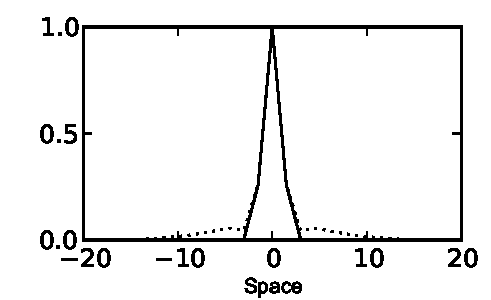
\includegraphics{./Figures/DisturbanceWidthEstimation.pdf}
\end{center}
\caption{{\bf Estimation of $\left(m\ast m \ast \gamma \right)\left(\boldsymbol \tau\right) $ width}. Values are normalised. True  and estimated values are shown with solid and dotted lines respectively.}
\label{fig:DisturbanceWidth}
\end{figure}
\newpage
\section*{Estimation of Kernel Support-II (With observation noise)}
The spatial relationship between consecutive observations is governed by the connectivity kernel. Therefore, the cross-correlation between consecutive observations is used to estimate the support of the connectivity kernel. The cross-correlation is defined as
\begin{align}
	R_{y_{t+1}y_t}(\boldsymbol{\tau})& =(y_{t+1} \star y_t)(\boldsymbol\tau) \nonumber \\
 &=\int_{\Omega} y_{t+1}(\mathbf{r}) y_t(\mathbf{r}+\boldsymbol{\tau}) d\mathbf{r},
\end{align}
where $\tau$ is the spatial shift. Now substituting for $y_{t+1}(\mathbf{r})$ 
\begin{equation}
	R_{y_{t+1}y_t}(\boldsymbol{\tau}) = \int_{\Omega}\left[ \int_{\Omega} m(\mathbf{r}-\mathbf{r}')v_{t+1}(\mathbf{r}')d\mathbf{r}'+\varepsilon_{t+1}(\mathbf r)\right]  y_t(\mathbf{r}+\boldsymbol{\tau}) d\mathbf{r}.
\end{equation}
Next  substituting in for $v_{t+1}(\mathbf{r}')$ gives
\begin{equation}
	R_{y_{t+1}y_{t+1}}(\boldsymbol{\tau}) = \int_{\Omega}\left[ \int_{\Omega} m(\mathbf{r}-\mathbf{r}')\left[ \xi v_t\left(\mathbf{r}'\right) + 
	T_s g_t(\mathbf{r}') 
	+ e_t\left(\mathbf{r}'\right)\right] d\mathbf{r}' +\varepsilon_{t+1}(\mathbf{r})\right] y_{t}(\mathbf{r}+\boldsymbol{\tau}) d\mathbf{r}.
\end{equation}
The cross-correlation is simplified by recognizing that 
\begin{align}
	\int_{\Omega}\int_{\Omega} m(\mathbf{r}-\mathbf{r}')&\xi v_t(\mathbf{r}')d\mathbf{r}'y_t(\mathbf{r}+\boldsymbol{\tau}) d\mathbf{r} = \nonumber \\ 
 &\xi \left(R_{y_ty_t}(\boldsymbol{\tau})-n_y\sigma_{\epsilon}^2  \delta_{K}\left(\boldsymbol\tau\right)\right),
\end{align}
where $\delta_{K}\left(.\right)$ denotes Kronecker delta. Also  
\begin{align}
	\beta(\boldsymbol{\tau}) &= \int_{\Omega}\int_{\Omega} m(\mathbf{r}-\mathbf{r}') e_t(\mathbf{r}') d\mathbf{r}'y_t(\mathbf{r}+\boldsymbol{\tau}) d\mathbf{r}=0 %\\
	% &= \int_{\Omega}\int_{\Omega} m(\mathbf{r}-\mathbf{r}') e_t(\mathbf{r}') d\mathbf{r}' y_t(\mathbf{r}+\boldsymbol{\tau}) d\mathbf{r}	
\end{align}
giving 
\begin{align}
	R_{y_{t+1}y_t}(\boldsymbol{\tau}) &= \xi \left(R_{y_ty_t}(\boldsymbol{\tau})-\sigma_{\epsilon}^2  \delta_{K}\left(\boldsymbol\tau\right)\right)\nonumber \\
	&+ T_s \int_{\Omega}\int_{\Omega} m(\mathbf{r}-\mathbf{r}')  g_t(\mathbf{r}') d\mathbf{r}' y_t(\mathbf{r}+\boldsymbol{\tau}) d\mathbf{r}.
\end{align}
Rearranging and substituting  for $g_t(\mathbf{r}')$ gives
\begin{align}
	R_{y_{t+1}y_t}(\boldsymbol{\tau}) &-\xi \left(R_{y_ty_t}(\boldsymbol{\tau})-\sigma_{\epsilon}^2  \delta_{K}\left(\boldsymbol\tau\right)\right) = T_s \int_{\Omega}\int_{\Omega} m(\mathbf{r}-\mathbf{r}') \nonumber \\
	&\times \int_{\Omega} w(\mathbf{r}'-\mathbf{r}'') f\left(v_t(\mathbf{r}'')\right)d\mathbf{r}'' d\mathbf{r}' y_t(\mathbf{r}+\boldsymbol{\tau}) d\mathbf{r}. 
\end{align}  
Using the commutativity property of convolution, the order can be rearranged to
\begin{align}
	R_{y_{t+1}y_t}(\boldsymbol{\tau})&-\xi \left(R_{y_ty_t}(\boldsymbol{\tau})-\sigma_{\epsilon}^2  \delta_{K}\left(\boldsymbol\tau\right)\right) =  T_s \int_{\Omega}\int_{\Omega} w(\mathbf{r}-\mathbf{r}') \nonumber \\
	&\times \int_{\Omega} m(\mathbf{r}'-\mathbf{r}'') f\left(v_t(\mathbf{r}'')\right) d\mathbf{r}'' d\mathbf{r}' y_t(\mathbf{r}+\boldsymbol{\tau}) d\mathbf{r}.
\end{align}
Next, the nonlinear function $f(\cdot)$ is approximated by the simple linear relationship
\begin{equation}
	f\left(v_t(\mathbf{r})\right) \approx \varsigma v_t(\mathbf{r})
\end{equation} 
giving
\begin{align}
	R_{y_{t+1}y_t}(\boldsymbol{\tau})&-\xi R_{y_ty_t}(\boldsymbol{\tau}) =  \varsigma T_s \int_{\Omega}\int_{\Omega} w(\mathbf{r}-\mathbf{r}') \nonumber \\
	&\times \int_{\Omega} m(\mathbf{r}'-\mathbf{r}'')  v_t(\mathbf{r}'') d\mathbf{r}'' d\mathbf{r}' y_t(\mathbf{r}+\boldsymbol{\tau}) d\mathbf{r},
\end{align}
which simplifies to
\begin{align}
	R_{y_{t+1}y_t}(\boldsymbol{\tau})-\xi \left(R_{y_ty_t}(\boldsymbol{\tau})-\sigma_{\epsilon}^2  \delta_{K}\left(\boldsymbol\tau\right)\right)& =  \varsigma T_s \int_{\Omega}\int_{\Omega} w(\mathbf{r}-\mathbf{r}')\left[ y_t(\mathbf{r}')-\varepsilon_t(\mathbf r')\right]  d\mathbf{r}' \times y_t(\mathbf{r}+\boldsymbol{\tau}) d\mathbf{r} \nonumber \\
	&=\varsigma T_s \int_{\Omega}\int_{\Omega} w(\mathbf{r}-\mathbf{r}') y_t(\mathbf{r}') d\mathbf{r}' \times y_t(\mathbf{r}+\boldsymbol{\tau}) d\mathbf{r} \nonumber \\
        &-\varsigma T_s \int_{\Omega}\int_{\Omega} w(\mathbf{r}-\mathbf{r}')\varepsilon_t(\mathbf r') d\mathbf{r}' \times y_t(\mathbf{r}+\boldsymbol{\tau}) d\mathbf{r}
\end{align}
This can be written in a compact form as
\begin{align}
	R_{y_{t+1}y_t}(\boldsymbol{\tau})-\xi \left(R_{y_ty_t}(\boldsymbol{\tau})-\sigma_{\epsilon}^2  \delta_{K}\left(\boldsymbol\tau\right)\right)& = \varsigma T_s(w\ast y_t)(\boldsymbol\tau)\star y_t(\boldsymbol\tau) \nonumber \\
&- \varsigma T_s(w\ast \varepsilon_t)(\boldsymbol\tau)\star y_t(\boldsymbol\tau)
\end{align}
A property of cross-correlation and convolution is $(a \ast b) \star c = a(-)\ast(b \star c)$, so we can write
\begin{align}
	R_{y_{t+1}y_t}(\boldsymbol{\tau}) -\xi \left(R_{y_ty_t}(\boldsymbol{\tau})-\sigma_{\epsilon}^2  \delta_{K}\left(\boldsymbol\tau\right)\right)& = \varsigma T_s w(-\boldsymbol\tau) \ast (y_t\star y_t)(\boldsymbol\tau)\nonumber\\
&-\varsigma T_s w(-\boldsymbol\tau) \ast (\varepsilon_t\star y_t)(\boldsymbol\tau)
\end{align}
In a case where connectivity kernel is isotropic $ w(-\boldsymbol\tau)= w(\boldsymbol\tau)$ and we have
\begin{align}
	R_{y_{t+1}y_t}(\boldsymbol{\tau}) -\xi \left(R_{y_ty_t}(\boldsymbol{\tau})-\sigma_{\epsilon}^2  \delta_{K}\left(\boldsymbol\tau\right)\right)& = \varsigma T_s (w\ast R_{y_ty_t})(\boldsymbol\tau)-\varsigma T_s \sigma^2_{\varepsilon}w(\boldsymbol\tau) 
\end{align}
The solution of the above equation for the connectivity kernel is a deconvolution. This can be approached from a number of different standpoints. The simplest solution is to use the convolution theorem and find the solution by 
\begin{equation}
	w(\boldsymbol{\tau}) = \frac{1}{\varsigma T_s}\mathcal{F}^{-1}\left\{\frac{\mathcal{F}\left(R_{y_{t+1}y_t}(\boldsymbol{\tau})\right)}{\mathcal{F}\left(R_{y_ty_t}(\boldsymbol{\tau})-\sigma^2_{\varepsilon}\delta_K(\boldsymbol\tau)\right)}-\xi\right\}.
\end{equation}

Alternatively, the convolution can be written as a system of linear equations by forming the convolution (Toeplitz) matrix. The solution of the convolution equation for $w(\cdot)$ can then be found by either inverting the convolution matrix or directly solving the system of equations. Directly solving the system is the most numerically stable and less computationally demanding then inverting the convolution matrix. 
\newpage
\section*{Estimation of Disturbance Support-II (Noise Free)}
The spatial correlation between observations at a given time is governed by the disturbance covariance function. Therefore, the correlation between observations at each time is used to estimate the support of the disturbance covariance function. The auto-correlation is defined as
\begin{equation}
	R_{y_{t+1}y_{t+1}}(\boldsymbol{\tau}) = \int_{\Omega} y_{t+1}(\mathbf{r}) y_{t+1}(\mathbf{r}+\boldsymbol{\tau}) d\mathbf{r},
\end{equation}
where $\tau$ is the spatial shift. Now substituting 
\begin{equation}\label{eq:ObservationEquation}
	y_t(\mathbf{r}) = \int_{\Omega} { m\left(\mathbf{r}-\mathbf{r}'\right) v_t\left(\mathbf{r}'\right) \, d\mathbf{r}'} + \varepsilon_t(\mathbf{r}_n), 
\end{equation}
for  $y_{t+1}(\mathbf{r})$ \parham{and assuming noise-free observations} gives 
\begin{equation}
	R_{y_{t+1}y_{t+1}}(\boldsymbol{\tau}) = \int_{\Omega}\int_{\Omega} m(\mathbf{r}-\mathbf{r}')v_{t+1}(\mathbf{r}')d\mathbf{r}' y_{t+1}(\mathbf{r}+\boldsymbol{\tau}) d\mathbf{r}.
\end{equation}
Next the equation
\begin{equation}
	\label{eq:DiscreteTimeModel} 
	v_{t+1}\left(\mathbf{r}\right) = 
	\xi v_t\left(\mathbf{r}\right) + 
	T_s \int_\Omega { 
	    w\left(\mathbf{r},\mathbf{r}'\right)
	    f\left(v_t\left(\mathbf{r}'\right)\right) 
	\, d\mathbf{r}'} 
	+ e_t\left(\mathbf{r}\right), 
\end{equation}
is substituted in for  $v_{t+1}(\mathbf{r}')$ giving 
\begin{align}
	R_{y_{t+1}y_{t+1}}(\boldsymbol{\tau}) &= \int_{\Omega}\int_{\Omega} m(\mathbf{r}-\mathbf{r}')\left(\xi v_t(\mathbf{r}') +  T_s g_t(\mathbf{r}')\right. \nonumber \\
	&+ \left. e_t(\mathbf{r}')\right) d\mathbf{r}' y_{t+1}(\mathbf{r}+\boldsymbol{\tau}) d\mathbf{r}. 
\end{align}
The auto-correlation is simplified by noting that
\begin{align}
	\int_{\Omega}\int_{\Omega} m(\mathbf{r}-\mathbf{r}')&\xi v_t(\mathbf{r}')d\mathbf{r}'y_{t+1}(\mathbf{r}+\boldsymbol{\tau}) d\mathbf{r} = \nonumber \\ 
 &\xi R_{y_ty_{t+1}}(\boldsymbol{\tau}),
\end{align}
giving
\begin{align}\label{eq:Auto&Cross}
	R_{y_{t+1}y_{t+1}}(\boldsymbol{\tau}) &= \xi R_{y_ty_{t+1}}(\boldsymbol{\tau}) \nonumber \\
	&+ T_s \int_{\Omega}\int_{\Omega} m(\mathbf{r}-\mathbf{r}')  g_t(\mathbf{r}') d\mathbf{r}' y_{t+1}(\mathbf{r}+\boldsymbol{\tau}) d\mathbf{r} \nonumber \\
	&+\int_{\Omega}\int_{\Omega} m(\mathbf{r}-\mathbf{r}')e_t(\mathbf{r}')d\mathbf{r}'y_{t+1}(\mathbf{r}+\boldsymbol{\tau}) d\mathbf{r}.
\end{align}
Substituting in equation
\begin{equation}
	\label{eq:RateBasedInteractions} g\left( \mathbf{r},t \right) = \int_\Omega {w\left( \mathbf{r},\mathbf{r}' \right)f\left( v\left( \mathbf{r}',t \right) \right)\, d\mathbf{r}'}, 
\end{equation}
for $g_t(\mathbf{r}')$, the second term in \eqref{eq:Auto&Cross} gives
\begin{align}
	\text{term2} = T_s \int_{\Omega}\int_{\Omega} m(\mathbf{r}-\mathbf{r}') 
	\times \int_{\Omega} w(\mathbf{r}'-\mathbf{r}'') f\left(v_t(\mathbf{r}'')\right)d\mathbf{r}'' d\mathbf{r}' y_{t+1}(\mathbf{r}+\boldsymbol{\tau}) d\mathbf{r}. 
\end{align} 
Using the commutativity property of convolution, the order can be rearranged to
\begin{align}
	\text{term2}  =  T_s \int_{\Omega}\int_{\Omega} w(\mathbf{r}-\mathbf{r}')
	\times \int_{\Omega} m(\mathbf{r}'-\mathbf{r}'') f\left(v_t(\mathbf{r}'')\right) d\mathbf{r}'' d\mathbf{r}' y_{t+1}(\mathbf{r}+\boldsymbol{\tau}) d\mathbf{r}.
\end{align}
Next, the nonlinear function $f(\cdot)$ is approximated by the simple linear relationship
\begin{equation}
	f\left(v_t(\mathbf{r})\right) \approx \varsigma v_t(\mathbf{r})
\end{equation} 
giving
\begin{align}
	\text{term2} =  \varsigma T_s \int_{\Omega}\int_{\Omega} w(\mathbf{r}-\mathbf{r}') 
	\times \int_{\Omega} m(\mathbf{r}'-\mathbf{r}'')  v_t(\mathbf{r}'') d\mathbf{r}'' d\mathbf{r}' y_{t+1}(\mathbf{r}+\boldsymbol{\tau}) d\mathbf{r},
\end{align}
which simplifies to
\begin{align}
	\text{term2}=  \varsigma T_s \int_{\Omega}\int_{\Omega} w(\mathbf{r}-\mathbf{r}')y_t(\mathbf{r}') d\mathbf{r}' 
	\times y_{t+1}(\mathbf{r}+\boldsymbol{\tau}) d\mathbf{r}
\end{align}
A property of cross-correlation and convolution is $(a \ast b) \star c = a(-)\ast(b \star c)$, so we can write
\begin{align}
	\text{term2}&= \varsigma T_s \int_{\Omega} w(\boldsymbol{\tau}-\boldsymbol{\tau}') 
	\times \int_{\Omega} y_t(\mathbf{r}) y_{t+1}(\mathbf{r}+\boldsymbol{\tau}') d\mathbf{r}d\boldsymbol{\tau}' \nonumber \\
	&= \varsigma T_s \int_{\Omega} w(\boldsymbol{\tau}-\boldsymbol{\tau}') R_{y_ty_{t+1}}(\boldsymbol{\tau}')d\boldsymbol{\tau}' \nonumber \\
	&=\varsigma T_s \left(w \ast R_{y_ty_{t+1}} \right)(\boldsymbol{\tau})
\end{align}
the third term in \eqref{eq:Auto&Cross} can be simplified as
\begin{align}\label{eq:term3}
\text{term3}&=\int_{\Omega}\int_{\Omega} m(\mathbf{r}-\mathbf{r}')e_t(\mathbf{r}')d\mathbf{r}'y_{t+1}(\mathbf{r}+\boldsymbol{\tau})  d\mathbf{r} \nonumber \\
&=\int \left(m \ast e_t\right)(\mathbf r)\left(m\left(\mathbf{r}+\boldsymbol\tau\right) \ast \left[\xi v_t\left(\mathbf{r}+\boldsymbol\tau\right) + 
	T_s \varsigma \left(w \ast v_t\right)(\mathbf r + \boldsymbol \tau)
	+ e_t\left(\mathbf{r}+\boldsymbol{\tau}\right) \right] \right)d\mathbf r \nonumber \\
	&=\int\left(m \ast e_t\right)(\mathbf r)\left(m \ast e_t\right)(\mathbf r+\boldsymbol\tau)d\mathbf r
\end{align}
Note that other terms in \ref{eq:term3} are zero.A property of cross-correlation and convolution is $(a \ast b) \star (a \ast b)=(a \star a)\ast(b \star b)$, so we can write
\begin{align}
 \int\left(m \ast e_t\right)(\mathbf r)\left(m \ast e_t\right)(\mathbf r+\boldsymbol\tau)d\mathbf r&=\left(m \ast e_t\right)(\boldsymbol\tau)\star\left(m \ast e_t\right)(\boldsymbol\tau) \nonumber \\
&=\left(m \star m\right)(\boldsymbol\tau)\ast\left(e_t \star e_t\right)(\boldsymbol\tau) \nonumber\\
&=m(-\boldsymbol\tau)\ast m(\boldsymbol\tau)\ast \gamma(\boldsymbol\tau) \nonumber \\
&=(m\ast m \ast \gamma)(\boldsymbol\tau)
\end{align}
Using expressions for term1, term2 and term3, $R_{y_{t+1}y_{t+1}}$ can be written as
\begin{align}
	R_{y_{t+1}y_{t+1}}(\boldsymbol{\tau})= \xi R_{y_ty_{t+1}}(\boldsymbol{\tau})+\varsigma T_s \left(w \ast R_{y_ty_{t+1}} \right)(\boldsymbol{\tau})+(m\ast m \ast \gamma)(\boldsymbol\tau)
\end{align}
Taking Fourier transform and rearranging we have
\begin{align}
 \mathcal F\left\lbrace (m\ast m \ast \gamma)(\boldsymbol\tau)\right\rbrace&= S_{y_{t+1}y_{t+1}}(\boldsymbol{\nu})-S_{y_{t}y_{t+1}}(\boldsymbol{\nu})-\varsigma T_s W(\boldsymbol{\nu}) \times S_{y_ty_{t+1}}(\boldsymbol{\nu}) \nonumber \\
\end{align}
and we have
\begin{align}
 W(\boldsymbol{\nu}) &=\frac{1}{\varsigma T_s}\left(\frac{S_{y_{t+1}y_t}(\boldsymbol{\nu}) -\xi S_{y_ty_t}(\boldsymbol{\nu})}{S_{y_ty_t}(\boldsymbol{\nu})}\right) \nonumber \\
&=\frac{1}{\varsigma T_s}\left(\frac{S_{y_{t+1}y_t}(\boldsymbol{\nu})}{S_{y_ty_t}(\boldsymbol{\nu})}-\xi\right).
\end{align}
Therefore
\begin{align}
 \mathcal F\left\lbrace (m\ast m \ast \gamma)(\boldsymbol\tau)\right\rbrace&= S_{y_{t+1}y_{t+1}}(\boldsymbol{\nu})-\left(1-\xi+\frac{S_{y_{t+1}y_t}(\boldsymbol{\nu})}{S_{y_ty_t}(\boldsymbol{\nu})}\right)S_{y_{t}y_{t+1}}(\boldsymbol{\nu})
\end{align}
\newpage

\section*{Estimation of Disturbance Support-III (with Observation Noise)}
The spatial correlation between observations at a given time is governed by the disturbance covariance function. Therefore, the correlation between observations at each time is used to estimate the support of the disturbance covariance function. The auto-correlation is defined as
\begin{equation}
	R_{y_{t+1}y_{t+1}}(\boldsymbol{\tau}) = \int_{\Omega} y_{t+1}(\mathbf{r}) y_{t+1}(\mathbf{r}+\boldsymbol{\tau}) d\mathbf{r},
\end{equation}
where $\tau$ is the spatial shift. Now substituting 
\begin{equation}\label{eq:ObservationEquationNoisy}
	y_t(\mathbf{r}) = \int_{\Omega} { m\left(\mathbf{r}-\mathbf{r}'\right) v_t\left(\mathbf{r}'\right) \, d\mathbf{r}'} + \varepsilon_t(\mathbf{r}), 
\end{equation}
for  $y_{t+1}(\mathbf{r})$ gives 
\begin{equation}
	R_{y_{t+1}y_{t+1}}(\boldsymbol{\tau}) = \int_{\Omega}\left[ \int_{\Omega} m(\mathbf{r}-\mathbf{r}')v_{t+1}(\mathbf{r}')d\mathbf{r}' +\varepsilon_{t+1}(\mathbf{r})\right] y_{t+1}(\mathbf{r}+\boldsymbol{\tau}) d\mathbf{r}.
\end{equation}
Next the equation
\begin{equation}
	\label{eq:DiscreteTimeModelNoisy} 
	v_{t+1}\left(\mathbf{r}\right) = 
	\xi v_t\left(\mathbf{r}\right) + 
	T_s \int_\Omega { 
	    w\left(\mathbf{r},\mathbf{r}'\right)
	    f\left(v_t\left(\mathbf{r}'\right)\right) 
	\, d\mathbf{r}'} 
	+ e_t\left(\mathbf{r}\right), 
\end{equation}
is substituted in for  $v_{t+1}(\mathbf{r}')$ giving 
\begin{equation}
	R_{y_{t+1}y_{t+1}}(\boldsymbol{\tau}) = \int_{\Omega}\left[ \int_{\Omega} m(\mathbf{r}-\mathbf{r}')\left[ \xi v_t\left(\mathbf{r}'\right) + 
	T_s g_t(\mathbf{r}') 
	+ e_t\left(\mathbf{r}'\right)\right] d\mathbf{r}' +\varepsilon_{t+1}(\mathbf{r})\right] y_{t+1}(\mathbf{r}+\boldsymbol{\tau}) d\mathbf{r}.
\end{equation}
The auto-correlation is simplified by noting that
\begin{align}
	\int_{\Omega}\int_{\Omega} m(\mathbf{r}-\mathbf{r}')&\xi v_t(\mathbf{r}')d\mathbf{r}'y_{t+1}(\mathbf{r}+\boldsymbol{\tau}) d\mathbf{r} = \nonumber \\ 
 &\xi R_{y_ty_{t+1}}(\boldsymbol{\tau}),
\end{align}
and
\begin{align}
 \int_{\Omega}\varepsilon_{t+1}(\mathbf{r})y_{t+1}(\mathbf{r}+\boldsymbol{\tau}) d\mathbf{r}&= \nonumber \\
&=\int_{\Omega}\varepsilon_{t+1}(\mathbf{r})\left[(m \ast v_{t+1})(\mathbf r+\boldsymbol\tau)+ \varepsilon_{t+1}(\mathbf{r}+\boldsymbol{\tau})\right] d\mathbf{r} \nonumber \\
&=\int_{\Omega}\varepsilon_{t+1}(\mathbf{r}) \varepsilon_{t+1}(\mathbf{r}+\boldsymbol{\tau}) d\mathbf{r} \nonumber \\
&=\sigma_{\epsilon}^2\delta_K(\boldsymbol{\tau})
\end{align}
giving
\begin{align}\label{eq:Auto&CrossNoisy}
	R_{y_{t+1}y_{t+1}}(\boldsymbol{\tau}) &= \xi R_{y_ty_{t+1}}(\boldsymbol{\tau}) \nonumber \\
	&+ T_s \int_{\Omega}\int_{\Omega} m(\mathbf{r}-\mathbf{r}')  g_t(\mathbf{r}') d\mathbf{r}' y_{t+1}(\mathbf{r}+\boldsymbol{\tau}) d\mathbf{r} \nonumber \\
	&+\int_{\Omega}\int_{\Omega} m(\mathbf{r}-\mathbf{r}')e_t(\mathbf{r}')d\mathbf{r}'y_{t+1}(\mathbf{r}+\boldsymbol{\tau}) d\mathbf{r}+\sigma_{\epsilon}^2\delta_K(\boldsymbol{\tau}).
\end{align}
Substituting in equation
\begin{equation}
	\label{eq:RateBasedInteractions} g_t\left( \mathbf{r}\right) = \int_\Omega {w\left( \mathbf{r},\mathbf{r}' \right)f\left( v_t\left( \mathbf{r}'\right) \right)\, d\mathbf{r}'}, 
\end{equation}
for $g_t(\mathbf{r}')$, the second term in \eqref{eq:Auto&CrossNoisy} gives
\begin{align}
	\text{term2} = T_s \int_{\Omega}\int_{\Omega} m(\mathbf{r}-\mathbf{r}') 
	\times \int_{\Omega} w(\mathbf{r}'-\mathbf{r}'') f\left(v_t(\mathbf{r}'')\right)d\mathbf{r}'' d\mathbf{r}' y_{t+1}(\mathbf{r}+\boldsymbol{\tau}) d\mathbf{r}. 
\end{align} 
Using the commutativity property of convolution, the order can be rearranged to
\begin{align}
	\text{term2}  =  T_s \int_{\Omega}\int_{\Omega} w(\mathbf{r}-\mathbf{r}')
	\times \int_{\Omega} m(\mathbf{r}'-\mathbf{r}'') f\left(v_t(\mathbf{r}'')\right) d\mathbf{r}'' d\mathbf{r}' y_{t+1}(\mathbf{r}+\boldsymbol{\tau}) d\mathbf{r}.
\end{align}
Next, the nonlinear function $f(\cdot)$ is approximated by the simple linear relationship
\begin{equation}
	f\left(v_t(\mathbf{r})\right) \approx \varsigma v_t(\mathbf{r})
\end{equation} 
giving
\begin{align}
	\text{term2} &=  \varsigma T_s \int_{\Omega}\int_{\Omega} w(\mathbf{r}-\mathbf{r}') 
	\times \int_{\Omega} m(\mathbf{r}'-\mathbf{r}'')  v_t(\mathbf{r}'') d\mathbf{r}'' d\mathbf{r}' y_{t+1}(\mathbf{r}+\boldsymbol{\tau}) d\mathbf{r} \nonumber \\
&=\varsigma T_s \int_{\Omega}\int_{\Omega} w(\mathbf{r}-\mathbf{r}') 
	\times \left[y_t(\mathbf r')- \varepsilon_t(\mathbf r')\right]  d\mathbf{r}' y_{t+1}(\mathbf{r}+\boldsymbol{\tau}) d\mathbf{r}
\end{align}
which simplifies to
\begin{align}
	\text{term2}&=  \varsigma T_s \int_{\Omega}\int_{\Omega} w(\mathbf{r}-\mathbf{r}')y_t(\mathbf{r}') d\mathbf{r}' 
	\times y_{t+1}(\mathbf{r}+\boldsymbol{\tau}) d\mathbf{r} \nonumber \\
&=\varsigma T_s \int_{\Omega} (w\ast y_t)(\mathbf{r})\times y_{t+1}(\mathbf{r}+\boldsymbol{\tau}) d\mathbf{r} \nonumber \\
&=\varsigma T_s(w\ast y_t)(\boldsymbol{\tau}) \star  y_{t+1}(\boldsymbol{\tau})
\end{align}
A property of cross-correlation and convolution is $(a \ast b) \star c = a(-)\ast(b \star c)$, so we can write
\begin{align}
	\text{term2}&= \varsigma T_s(w\ast y_t)(\boldsymbol{\tau}) \star  y_{t+1}(\boldsymbol{\tau}) \nonumber \\
	&= \varsigma T_s w(-\boldsymbol\tau)\ast \left[  y_t(\boldsymbol{\tau}) \star  y_{t+1}(\boldsymbol{\tau})\right] \nonumber \\
	&=\varsigma T_s w(-\boldsymbol\tau)\ast R_{y_ty_{t+1}} (\boldsymbol{\tau}).
\end{align}
In the case where connectivity kernel is isotropic we have
\begin{align}
	\text{term2}&= \varsigma T_s (w \ast R_{y_ty_{t+1}}) (\boldsymbol{\tau}).
\end{align}
the third term in \eqref{eq:Auto&Cross} can be simplified as
\begin{align}\label{eq:term3Noisy}
\text{term3}&=\int_{\Omega}\int_{\Omega} m(\mathbf{r}-\mathbf{r}')e_t(\mathbf{r}')d\mathbf{r}'y_{t+1}(\mathbf{r}+\boldsymbol{\tau})  d\mathbf{r} \nonumber \\
&=\int \left(m \ast e_t\right)(\mathbf r)\left[m\left(\mathbf{r}+\boldsymbol\tau\right) \ast \left[\xi v_t\left(\mathbf{r}+\boldsymbol\tau\right) + 
	T_s \varsigma \left(w \ast v_t\right)(\mathbf r + \boldsymbol \tau)
	+ e_t\left(\mathbf{r}+\boldsymbol{\tau}\right) \right]+\varepsilon_{t+1}(\mathbf r+\boldsymbol\tau) \right]d\mathbf r \nonumber \\
	&=\int\left(m \ast e_t\right)(\mathbf r)\left(m \ast e_t\right)(\mathbf r+\boldsymbol\tau)d\mathbf r
\end{align}
Note that other terms in \ref{eq:term3Noisy} are zero.A property of cross-correlation and convolution is $(a \ast b) \star (a \ast b)=(a \star a)\ast(b \star b)$, so we can write
\begin{align}
 \int\left(m \ast e_t\right)(\mathbf r)\left(m \ast e_t\right)(\mathbf r+\boldsymbol\tau)d\mathbf r&=\left(m \ast e_t\right)(\boldsymbol\tau)\star\left(m \ast e_t\right)(\boldsymbol\tau) \nonumber \\
&=\left(m \star m\right)(\boldsymbol\tau)\ast\left(e_t \star e_t\right)(\boldsymbol\tau) \nonumber\\
&=m(-\boldsymbol\tau)\ast m(\boldsymbol\tau)\ast \gamma(\boldsymbol\tau) \nonumber \\
&=(m\ast m \ast \gamma)(\boldsymbol\tau)
\end{align}
Using expressions for term1, term2 and term3, $R_{y_{t+1}y_{t+1}}$ can be written as
\begin{align}
	R_{y_{t+1}y_{t+1}}(\boldsymbol{\tau})= \xi R_{y_ty_{t+1}}(\boldsymbol{\tau})+\varsigma T_s \left(w \ast R_{y_ty_{t+1}} \right)(\boldsymbol{\tau})+(m\ast m \ast \gamma)(\boldsymbol\tau)+\sigma_{\epsilon}^2\delta_K(\boldsymbol{\tau}).
\end{align}
Taking Fourier transform and rearranging we have
\begin{align}
 \mathcal F\left\lbrace (m\ast m \ast \gamma)(\boldsymbol\tau)\right\rbrace&= S_{y_{t+1}y_{t+1}}(\boldsymbol{\nu})-\xi S_{y_{t}y_{t+1}}(\boldsymbol{\nu})-\varsigma T_s W(\boldsymbol{\nu}) \times S_{y_ty_{t+1}}(\boldsymbol{\nu})-\sigma_{\epsilon}^2 
\end{align}
and we have
\begin{align}
 W(\boldsymbol{\nu}) &=\frac{1}{\varsigma T_s}\left(\frac{S_{y_{t+1}y_t}(\boldsymbol{\nu})}{S_{y_ty_t}(\boldsymbol{\nu})-\sigma_{\epsilon}^2}-\xi\right).
\end{align}
Therefore
\begin{align}
 \mathcal F\left\lbrace (m\ast m \ast \gamma)(\boldsymbol\tau)\right\rbrace&= S_{y_{t+1}y_{t+1}}(\boldsymbol{\nu})-\frac{S_{y_{t+1}y_t}(\boldsymbol{\nu})S_{y_{t}y_{t+1}}(\boldsymbol{\nu})}{S_{y_ty_t}(\boldsymbol{\nu})-\sigma_{\epsilon}^2}-\sigma_{\epsilon}^2
\end{align}

\section*{Appendix}
\subsection*{Convolution and Correlation}
To show  
\begin{equation}
(a \ast b)(\boldsymbol \tau) \star (a \ast b)(\boldsymbol\tau)=(a \star a)(\boldsymbol\tau)\ast(b \star b)(\boldsymbol\tau)
\end{equation}
we note that cross-correlation function is related to the convolution by 
\begin{equation}
 \left(a \star b\right)\left(\tau\right)= a\left(-\tau \right)\ast b\left(\tau\right).
\end{equation}
Therefore, we can write
\begin{align}
 (a \ast b)(\boldsymbol \tau) \star (a \ast b)(\boldsymbol\tau)&=(a \ast b)(\boldsymbol -\tau) \ast (a \ast b)(\boldsymbol\tau) \nonumber \\
&=a(-\boldsymbol\tau)\ast a(\boldsymbol\tau) \ast b(-\boldsymbol\tau)\ast b(\boldsymbol\tau) \nonumber \\
&=(a \star a)(\boldsymbol\tau)\ast(b \star b)(\boldsymbol\tau)
\end{align}
\bibliographystyle{plain}
\bibliography{}
\end{document}
